\documentclass[12pt]{article}

%\usepackage[table]{xcolor}
\usepackage{makeidx}
\usepackage[normalem]{ulem}
\usepackage{multirow}
\usepackage{multicol}
\usepackage{natbib}
\usepackage{graphicx}
\usepackage{longtable}
\usepackage[table,xcdraw]{xcolor}
\usepackage{tabularx}
\usepackage[paperwidth=595pt,paperheight=841pt,top=72pt,right=72pt,bottom=72pt,left=72pt]{geometry}

\begin{document}

\title{\Huge Silver Team \\ NavUP \\ Software Requirements Specification}
\author{\Large Bongani Tshela, 14134790 \\
		\Large Schae Ind, 14058104 \\
		\Large Merissa Joubert, 15062440 \\
		\Large Simon Johannes du Plooy, 12070794 \\
		\Large Henry Wandera, 17253129 \\
		\Large Monkeli Dilapisho, 15074260 \\
		\Large Nardus van der Vyver, 15012698}
\date{\today}
\maketitle

\newpage
\tableofcontents
\newpage






\pagebreak

\section{Introduction}
	\subsection{Purpose}

	The purpose of this document (Requirements Specification Document) is to outline the requirements of the NavUP application that is to be designed and built. This document will specify our requirements of the product, related to performance, external and internal interface, as well as provide the functional requirements and design constraints to be met. The requirements will help define and determine user expectations, thus allowing the team to build an effective and functional application. 

\vspace{\baselineskip}
The Requirements Specification Document will be used as an official document between the client(s) and the designers/engineers of the software to ensure that both parties understand the requirements and capabilities. This document will serve to outline the user needs and expectations for the application, as well as offer guidelines for the builders of the software. This document will help to determine what must be included in the software for it to fulfil its desired purpose.


	\subsection{Scope}

	The product to be built is called NavUP. The product will act as a navigation system for the University of Pretoria. NavUP will be a mobile application that will allow the user to navigate both indoors and outdoors at the University of Pretoria, as well as choose from a series of available routes to a set destination, based on the user’s restrictions and requirements. The application will allow the user to interact with it, much like a GPS would, thus enabling the user to view pedestrian congestion, get directions, and find and save locations. The software will also provide the user with functional, cultural and historical information about their surroundings, as well as allow them to find and navigate to a place based on said information.
\vspace{\baselineskip}

NavUP will function as a fully dedicated University of Pretoria navigation system, as well as an information application, providing valuable information on the location and history of, as well as routes to the buildings located on the campus. The software will be used to provide people who are unfamiliar with the campus with the location of specific buildings and lecture halls, and the various routes that can be used to navigate to them. NavUP will provide users with the ability to navigate on the campus based on specific restrictions or requirements, such as only showing routes where wheelchair access is available. NavUP hopes to improve class punctuality by detailing faster routes and showing pedestrian congestion. The application also hopes to minimise frustration with new students and visitors to the campus by allowing them to navigate effectively and independently across the grounds and in the buildings. NavUP will be a valuable tool in helping students and visitors alike learn about the rich cultural and architectural history of the many buildings at the University of Pretoria.

	\subsection{Definitions, Acronyms and Abbreviations}
		\subsubsection{Definitions:}
		\textbf{Requirements} – “descriptions of the services that a software system must provide” \textit{(CS2 Software Engineering note 2, 2004)} \\
		\\ \textbf{Software Requirements Specification} – Also known as a ‘Requirements Specification Document’ describes the features and intended purpose of a software application \textit{(Rouse, 2007)} \\
		\\ \textbf{Functional Requirements} – specifies something the system “should do” or a “behaviour or function” the system should have \textit{(Eriksson, 2012)} \\
		\\ \textbf{Constraint} – Something that restricts your “freedom to do what you want” \textit{(Longman Dictionary of Contemporary English, n.d.)} \\
		\\ \textbf{NavUP} – The navigational application product that is to be built


		\subsubsection{Acronyms:}
		\textbf{UP} – University of Pretoria\\
		\\ \textbf{SRS} – Software Requirements Specification


		\subsubsection{Abbreviations:}
		\textbf{App} - Aplication


	\subsection{References}

CS2 Software Engineering note 2. (2004). \textit{CS2Ah Autumn 2004}, 1. \\\\
Eriksson, U. (2012, April 5). \textit{Functional vs Non Functional Requirements. Retrieved from ReQtest}: http://reqtest.com/requirements-blog/functional-vs-non-functional-requirements/ \\\\
Longman Dictionary of Contemporary English. (n.d.). constraint. Retrieved from Longman Dictionary of Contemporary English: http://www.ldoceonline.com/dictionary/constraint \\\\
Morkel Theunissen, Vreda Pieterse, Stacey Omeleze, Emilio Singh. (2017, February). COS301 - \textit{Software Engineering. Retrieved from Computer Science}: http://www.cs.up.ac.za/courses/COS301 \\\\
Rouse, M. (2007, February). \textit{Software Requirements Specification (SRS).} Retrieved from Search Software Quality: http://searchsoftwarequality.techtarget.com/definition/software-requirements-specification





	\subsection{Overview}
This document will highlight the requirements and user expectations. It will provide a detailed overview of the product, as well as the context of the product and how it interfaces and works with other components of the entire system. The characteristics and limits of the product’s memory availability will also be discussed.
\vspace{\baselineskip}
The functions, characteristics and constraints of NavUP will be touched upon, along with specific requirements; namely, external interface, functional, performance, design and software system requirements.
\vspace{\baselineskip}
The product will be looked at in terms of what is necessary and what is possible for the specific target market it aims to satisfy.

\section{Overall Description}
\subsection{Product Perspective}

\subsubsection{System Interfaces}
The System Interface is basically all the internal interfaces between the application (software) and everything else within the bigger system.
The System Interface includes all the interfaces and their functionality to accomplish the system requirement, interfaces include user (screen), hardware (mobile device), software (NavUP) and communications (Wi-Fi) – interfaces.

\subsubsection{User Interfaces}
The User Interfaces include:
The NavUP application with all its interactive parts (Buttons, scroll bars, search bars, links etc.)
The NavUP application in the form of how it is embodied on the screen.
The keyboard used in-app to type a destination or so on.
The touch screen used in order to navigate the application effectively.\\
*The User Interface entails accepting input via devices like the touch screen or keyboard in order to provide output in the form of a Graphical User Interface on the portable device of choice. The GUI (Graphical User Interface) provides the output that will guide the user on his/her journey through campus. 

\subsubsection{Hardware Interfaces}
The Hardware Interfaces include:
The mobile device of choice (Phone/Tablet).
*not taking pc or laptops into consideration because of the mobile nature of the app.
Hardware like the screen (used to display the user interface of the application and record user actions like typing and selecting).
The mobile devices’ network receiver used to connect to campus Wi-Fi.
The accelerometer of the phone that can be used to measure how fast or where the person is walking while in-app.
The devices memory(primary and secondary)\\
*The Hardware Interface is one of the core parts of the project (The input/output device), as the software product (NavUP) has to connect with the hardware components of the device. 

\subsubsection{Software Interfaces}
The Software Interfaces include:
The Mobile device OS (Operating System), that will handle all the requests made by the NavUP application.
The NavUP application that will run on the phone.\\
*The Software Interfaces will provide access to the mobile devices resources like the storage (saving locations in-app), CPU(processing any requests needed).

\subsubsection{Communications Interfaces}
The Communications Interfaces include:
The mobile devices’ network receiver (to connect to Wi-Fi) and program used to translate the signals received. 
The Wi-Fi sign on the mobile device that will give indication of signal strength and connectivity.\\
*The Communications Interface handles requests to and from the Wi-Fi and application server that will give the user the experience and output needed.


\begin{figure}[h!]
\centering
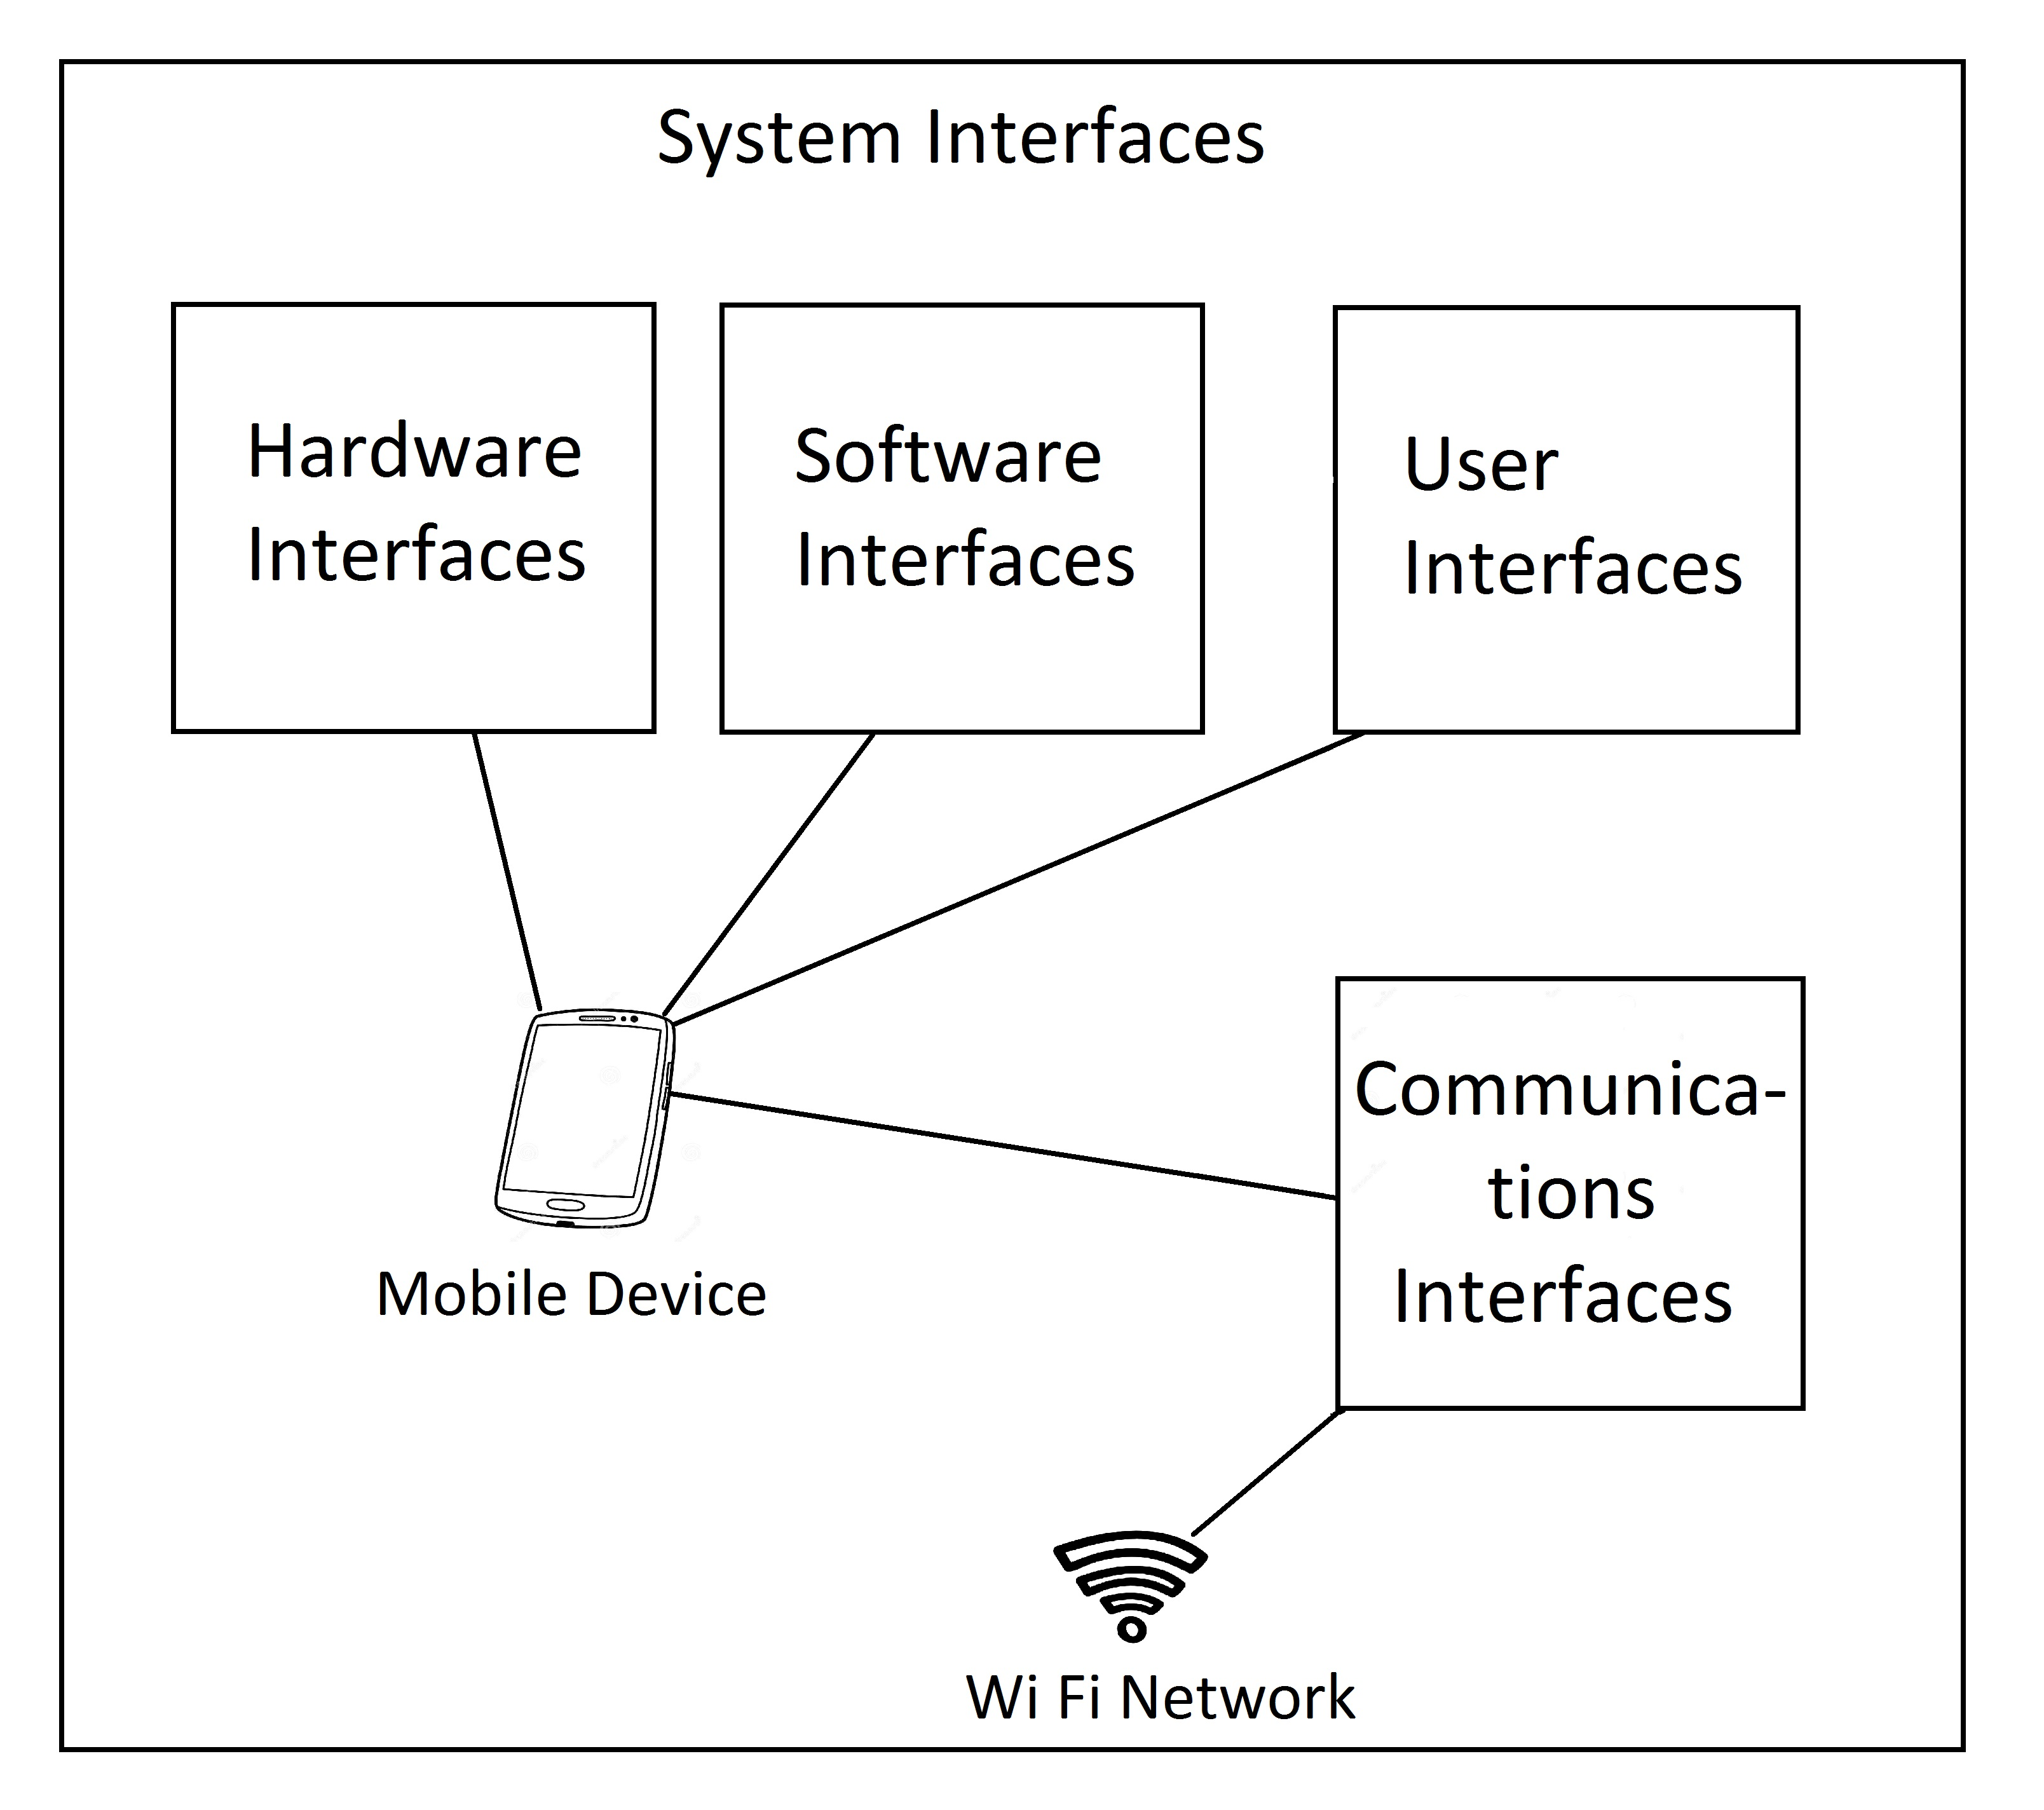
\includegraphics[scale=0.1]{BLockDiagram.jpg}
\caption{Block Diagram}
\label{fig:block diagram}
\end{figure}

\subsubsection{Memory}
\textbf{Primary Memory:}
The primary memory refers to the RAM (Random Access Memory) of the mobile device. 
The RAM is used to store information intended for immediate use within the app. 
A limit that primary storage brings is that it is volatile, so no in-app data can be stored and retrieved later.
Another limit is that RAM can vary in size, the bigger the size the better the app will perform (because more information can be stored and accessed quickly), but that is dependent on the various different mobile devices.\\\\
\textbf{Secondary Memory:}
The secondary memory includes the devices internal hard drive as well as external SD cards.
Secondary memory is where the program as well as the saved data (locations and other in-app details) is kept and stored on a long term basis. 
A limit of secondary storage is that it is much slower that primary memory and may cause the application to take a while to open.
Another limit is that the data stored can be gone if stored on SD card and the card is removed.
If the mobile device is broken or destroyed you will not be able to access your saved data and information.


\subsubsection{Operations}

%\paragraph{Operations}

%\begin{center}

This section describes the operation support systems.

		

The program will be required to, through the usage of mobile data or wifi networks, download and upload GIS information. It is possible to interlink the program with the Googlemaps.api as it is widely supported by most mobile devices.

		

Further and beyond the GIS interoperability the program will be required to implement a navigations system mapping best routes which might require the program to transform GIS information into data structures upon which shortest-path algorithms and algorithms of that nature can be implemented. It will therefore be required that a suitable high-level programming language be chosen for both ios devices and android devices, as they are the targeted operating systems.

		

		For ios devices the options are:

		\begin{list}{}{}

			

			\item ObjectiveC and C

			\item C++ using the XCode Platform

			\item OCaml

		\end{list} 

	

		For Android devices the options are:

			\begin{list}{}{}

				\item Java

				\item C and C++ using the Android Native Development Kit (NDK)

			\end{list}

	%\end{center}


\subsubsection{Site Adaptation Requirements}


This section describes requirements that are specific to data and initialization sequences for this product.

The initial data initialization sequence begins with the login and setting the user session as the user logs in. This information will be stored on a database system. From there the product should initialise the maps and updates content that might have been stored using cookies so as to give current real time information.

\subsection{Product Functions}


This section provides a summary of the product functions.

	

Provide a traditional navigation system. Which includes the functions of searching locations, saving locations, allowing the user to both use their current location as well as choose to input a location as a starting point. The system will need to be able to show both text and visual directions and include an interface for the visually impaired.

	

Furthermore the product will have the features of a sports fitness app, allowing registered users to compete for "rewards" based on the number of steps one has taken throughout a day, with this route being possibly mapped and recorded.

The interface shall include options to allow the user to view points of interest on the map as well as provide additional information about those points of interest.

\subsection{User Characteristics}
The following is a description of the characters we assume the user possesses/should
possess in order to fully utilize the product
This product is intended for a user who is currently studying at/visiting/working
at the University of Pretoria. The user is expected to have a basic understand-
ing of navigational systems in order to use the base functionality of the program
such as mapping the route from one place to another. For the other functionali-
ties such as the step counter/fitness section, the user would require a familiarity
with such systems. Do to the nature of the product the user need not have a
specifc educational level just a basic affinity towards maps technology.

\subsection{Constraints}
The following is a description of the restrictions upon the solution space.
The solution space is restricted by device (hardware and software) in the
sense that only devices with location services as well as the intended ios/android
operating systems will have access to the product. Due to the difference in op-
erating systems the programmer has the option of either implementing separate
systems which work in the same way in two different languages or using a com-
mon language such as Objective C/c++/C in order to write one system that
works on both kinds of devices. The latter has the draw back of not being
able to fully utilize each OS's intricate prowess and creating extra work for the
programmer to develop a more modular software. The programmer is also limited by the mobile data/wifi data consumption limit that one should place on the product. With the intended target market in mind, as far as possible, the product should be developed such that it can run in the background without
being resource expensive. Further than the mobile data/wifi data resource the programmer has to consider the computational expense as well as the memory expense.

\subsection{Assumptions and Dependencies}
\begin{list}{Assumption:}{}
	\item The user possesses a smart phone.
	\item The user has a desire to navigate through campus faster.
	\item The user has a desire to participate in the fitness aspect of the
app.
\end{list}

\begin{list}{Dependency:}{}
	\item A map/blueprint of the internals of the buildings as well as a
map of the University of Pretoria.
	\item Access to the University of Pretoria Wifi network so as to create
heat maps of devices currently linked so as to show foot traffic.
	\item Access to a hosting service on which the product can host the
database and other user information.
\end{list}

%///////////////////////////////////////bongani


%\title{}



%\maketitle
\section{Specific Requirements}

\subsection{External Interface Requirements}

This section provides a detailed description of all inputs into and outputs from

the system. It also gives a description of the hardware, software and

communication interfaces and provides basic prototypes of the user interface.



\subsubsection{User Interface}



{\raggedright

When users open the app, they will find a log-in page where they can enter they're log-in details if they're not first time users. First time users will have to click the register link found on the log in page to register as users of the app or if a user does not want to register, they can continue as guests. Users must note that the privileges of registered will not be the same as those of guests (explained below). 

}



{\raggedright

\uline{Guest Users:}}



{\raggedright

The app will cater for guest users and registered users. Guest users will not have to log in (will use the app as guests). However, when one logs in as a guest, no information about the user will be stored in the database and they will have access to information that is not registered users sensitive (e.g adverts). The guest users will only be able to use the navigation.

}



{\raggedright



}



{\raggedleft

\uline{Registered users:}}



{\raggedright

Registered users will find an extra module(page) where they will be able to add they're favourite events or buildings on campus. They will also be able to import they're timetables after which the app will notify them classes.

}



{\raggedright

\uline{Navigation page:}}



The app will find the users current location (using GPS/network provider info/WI-FI signals). At the navigation page, users will find a single form on which the users will have to submit/enter the desired location.(see picture below for example)



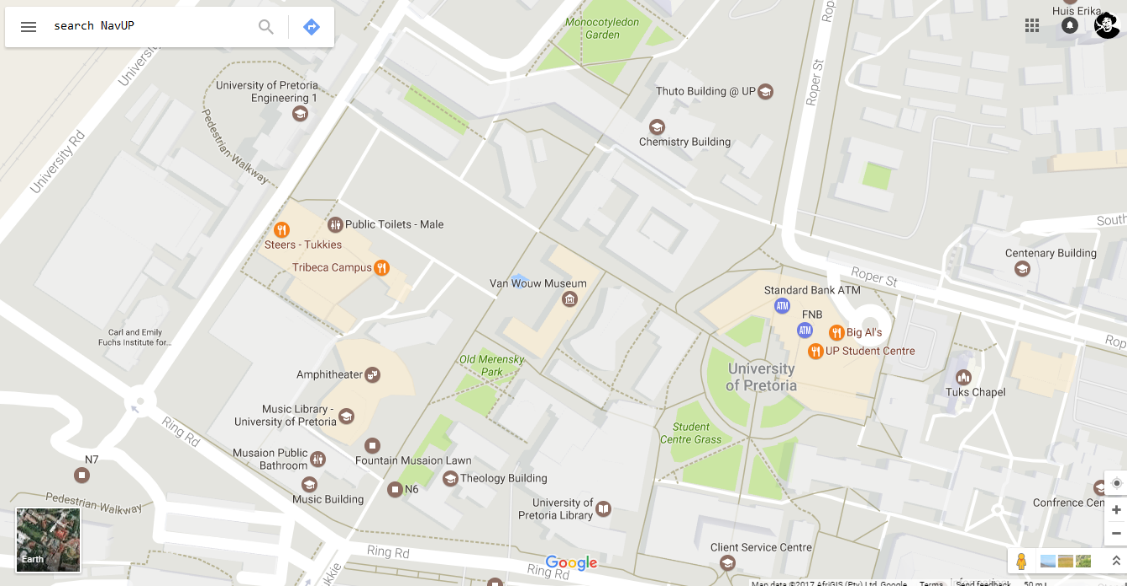
\includegraphics{1.png}



After users have entered the desired location, the app will locate and navigate them to that location. 







\subsubsection{Hardware Interface}

{\raggedright

Operation systems or platforms supported: Android, IOS and browsers that support

HTML, CSS, Java-Script (and other web-development and scripting languages). The

NavUP app will depend on the UP Wi-Fi for buildings to be located and devices

using the NavUP app must have Wi-Fi sensors.

The app will also support all types of devices that run the platforms IOS and Android(mobile phones, tablets, phablets). The devices accelerometer can be used to measure how fast or where the person is walking while in-app.

}



\subsubsection{Software Interface}

{\raggedright

The app is to be developed for Android, IOS and Web. Android studio will be used

to develop for android (The API Android.location will be used amongst others),

Xcode will id used to develop for ISO and web-development and scripting languages

will be used for the Web app part.

}



{\raggedright



\uline {Software needed or to be implemented:}

}



{\raggedright

Database of users information (SQL+ or MongoDB)

}



{\raggedright

Data structures to store buildings, access points, routs and shortest paths.

}



{\raggedright

Real time data analysis and data streaming tools

}



\subsubsection{Communication Interface}

{\raggedright

When the desired location is entered, the coordinates will be sent to the

back-end software/data structure for the app to locate then give directions. The

NavUP app may have a web based server, which will be created using PHP. The

server will retrieve the needed information from the database/data structure. The

HTTP server will use a push protocol to push notifications of updates onto the

user's applications. The Wi-Fi sign on the mobile device that will give indication of signal strength and connectivity.The Communications Interface handles requests to and from the Wi-Fi and application server that will give the user the experience and output needed.Furthermore, whenever a user opens the NavUP app from their

phone, a pull protocol will be used to retrieve and sync the latest updates from

the server.

}
%////////////////////////////merissa





\subsection{Functional Requirements}
\begin{longtable}{|p{.10\textwidth}| p{.20\textwidth} | p{.60\textwidth} |}

\hline

REQID& Section & Requirement Definition \\

\hline

1.& Login and Authentication & The system shall provide login facilities that will allow different users to log into different interfaces based on their status. For example students will be able to access the student navigation system while third party members will be able to access the rewards interface for adjustments, settings and push notifications.  \\

\hline

1.2& Login and Authentication   & The system will have non-login functionality for guests. \\

\hline

2.1& Input & The system shall provide a searching interface that will enable users to search for: venues, events, sporting facilities, historical landmarks, day houses, faculty houses and other points of interest  \\

\hline

2.2& Input  & The system shall provide a timetable import function in order to enable students to find their classes on time.  \\

\hline

2.3& Input  & The system shall provide users with different route planning options in order to optimize travelling experience. Route options include: fastest route, shortest route, least congested route and scenic route. \\

\hline

2.4& Input  & The system shall be able to receive voice commands in order to facilitate users with visual impairments.\\

\hline

3.1& Output & The system shall notify users of : upcoming classes, upcoming events\\

\hline

3.2& Output &The system shall notify users when they have reached their destination \\

\hline

3.3& Output & The system shall provide a navigation interface containing a map of the area surrounding the user and an indication of the user's position on campus\\

\hline

3.4& Output & The system shall have an option for verbal output in 2 major languages in order to aid users with visual impairments.\\

\hline

3.5& Output & The system shall include a series of vibrations that will enable the user to mute the system and still receive notifications.\\

\hline

3.6& Output & The system shall have vibrations that confirm interaction with the screen to aid visually impaired users.\\

\hline

3.7& Output & The system shall calculate and display the estimated travel time for the user's current route.\\

\hline

3.8& Output & The system shall give the user directions to the requested location both indoors and outdoors.\\

\hline

3.9& Output& The system shall provide users with quick predefined routes to the nearest ablution facilities, restaurants and shops.\\

\hline

3.10& Output& The system shall allow the user to access heat maps of campus in order to view congestion of the routes they are following.\\

\hline

4.1& Network Connection & The system shall use campus wifi access points to triangulate the position of the user and calculate routes.  \\

\hline

4.2& Network Connection & The system shall use cellular networks to triangulate the position of the user and calculate routes when the user is in an area with low or no wifi coverage.\\

\hline

4.3& Network Connection & The system shall use GPS to find the position of the user accurately and calculate routes precisely.\\
\hline

5.1& Data Storage & The system shall store user information in a user profile to enable profiling for push notifications.\\

\hline

5.2& Data Storage & The system shall store the steps taken and distance travelled by the user for use in reward systems and activities designed by third party users.\\

\hline

5.3& Data Storage & The system shall store a list of recently used routes for ease of access to the user and surveillance purposes.\\

\hline

5.4& Data Storage & The system shall cache the main campus map and all locations in order to minimize downloading of data and speed up navigation processes.\\

\hline

6.1& Data Analysis & The system will allow administrators to analyse stored data to produce statistical graphs and reports on student movement on campus.\\

\hline

6.2& Data Analysis & The system will allow administrators to view the number of students on campus at any point in time as well as the number of students in any class at any given point in time.\\

\hline

6.3& Data Analysis & The system will allow administrators to analyse individual user movement sand habits to sort users amongst general stereotypes in order to use push notifications.\\

\hline

7.1& Error Handling & The system will include off-line functionality in case of signal loss or disconnection from the network.\\

\hline

7.2& Error Handling & The system shall provide route recalculation and correction functionality in case of incorrect navigation.\\

\hline

7.3& Error Handling & The system shall allow users to add new personal locations. This is to cater for personal favourite leisure areas as well as any buildings that may be missed by the development team. \\

\hline

7.4& Error Handling & The system shall automatically save the state at selected time intervals in case of system failure for whatever reason.\\

\hline

7.5& Error Handling & The system shall include saved state recall functionality to enable users to resume their route after a potential system failure.\\

\hline

8.1& Disabled Student support & The system shall include a special needs interface for visually impaired users.\\

\hline

8.2& Disabled Student support & The system shall include an easy access list of wheelchair friendly access points and routes to aid disabled users.\\

\hline

8.3& Disabled Student support & The system shall include adjustable interface settings to enable  the user to change settings based on their disabilities. These settings include : colour adjustments for colour blind users, sound adjustments for deaf users, touch sensitivity adjustments for users with physical disabilities.\\

\hline

9.1& Activities & The system shall include background activity modules that can be activated by the user if they wish.\\

\hline

9.2& Activities & The system shall include a list of entertainment routes that will allow the user to explore campus and learn about new locations they might not have known about.\\

\hline

9.3& Activities & The system shall include a list of exercise routes that the user can use to train on campus. These routes will also be used in an exercise mode that will contain training music and an optional coach to motivate runners.\\

\hline

9.4& Activities & The system shall include a diary in the user's profile where they will be able to view the special buildings and landmarks that they have visited.\\

\hline

9.5& Activities & The system shall have a group walk functionality that can be used to coordinate  and other group activities.\\ 

\hline

9.6& Activities & The system shall have access to a calender and use it to activate special holiday activities designed by the developing team. These include: Easter egg hunt, hidden valentines day cards for couples, Halloween themed ghost hunt and many more at the discretion of the developers.\\

\hline

9.7& Activities & The system shall provide users with the option of connecting their profiles to health applications like Shealth in order to improve their life styles.\\

\hline

10.1& Reward systems & The system shall use the step counter to notify the user when milestones like 1000 steps have been reached. This functionality can be used to reward users who walk often.\\

\hline

10.2& Reward systems & The system shall allow users to set goals based on the distances they walk daily, weekly and monthly. \\

\hline

10.1& Reward systems & The system shall keep track of how many classes the user attends and use this number to award the user when they attend classes consistently.\\

\hline

10.4& Reward systems& The system  shall keep track of the number of locations visited by the user and reward them when they have reached milestones like 5, 10 and more buildings at the discretion of the developing team.\\

\hline

11.1& Help &The system shall provide an instruction page where users will be able to learn how to use the application and find all the functionalities available to them.\\

\hline

11.2& Help& The system shall provide hints and tips in pop-ups that the user may activate or de-activate at their own discretion.\\

\hline

11.3& Help& The system shall make suggestions about better route options that are in line with set goals or traffic congestion when the user chooses a route.\\

\hline

12.1 &Navigation functionality & The system shall provide navigation functionality both indoors and out doors using the various networking capabilities mentioned.\\

\hline

12.2&Navigation functionality &The system shall use the user device's location services for accurate location prediction.\\

\hline





\caption{Detailed Functional Requirements} % needs to go inside longtable environment

\label{tab:NavUP Functional Requirements}

\end{longtable}






	\subsection{Performance Requirements}

	

	Since the application’s main feature is navigation, it goes without saying that it should be designed and optimized for mobile devices such as smart phones and tablets.  Thus we are limited by the amount of Memory and Processing power we would have at our disposal.  We also need to account for all the different mobile platforms, such as Apple IOS and Android to name a few.  It is possible to develop a hybrid application to accommodate the various platforms, however that could possibly limit the functionality available to us as opposed to developing a native application for all the major platforms.  

	

	Furthermore, seeing as how the application could possibly be running for hours in the background, it is imperative that the application not be heavily energy consuming.  This could mean being smart about how we handle the various types of connections the application would need, and how long/often a connection should be established.  

	

	There should also be a balance between the number of data processing being handled client and server side.  If only raw data is being fed to the client, it would need to expend more energy processing the data.  On the other hand, if all of the processing is handled server side, it would mean keeping a connection open for longer periods of time, which could result in massive amounts of network traffic, which would in turn only get worse with each new user added to the system.  Furthermore, it is also important to decide what parts of the data would be done client side versus server side.  Essentially you would want most of the heavy lifting be done server side, leaving the more basic work to be done client side, so as to use the memory, processing power, and battery power as efficiently as possible.   

	

	

	\subsection{Software System Attributes}

	

		\subsubsection{Reliability}

		The application will have to be accurate within the average person’s viewing distance, in other words, the user should be guided to within viewing distance of the desired destination.  Furthermore, the application’s resources, such as maps, location triangulation, etc., will have to be as updated as possible within reason, so as to ensure the user not be misled to an old or even non-existing venue.  

		

		One of the application’s desired functionality is to be able to indicate to the user the shortest/fastest path from their current location to their intended destination.  A possible method the application could utilize would be through crowd sourcing, in that other users’ general location be used to generate heat-maps to indicate congestion on a possible route.  Furthermore, the application could also be informed by the system of any possible construction taking place on a given route, which could also cause obstructions, adding to possible congestion levels, and would rather be avoided if at all possible.  

		

		\subsubsection{Availability}

		The application will rely heavily on an active connection to either a Wi-Fi connection for indoor navigation, or a GPS connection and/or Cellular connection for outdoors.  This will however not always be the case, therefore the application would have to make provisions in the event there are no connections available, or the signal is being blocked for whatever reason.  This could possibly be done by caching a reasonable amount of the map and current location, then when the signal drops, make use of the user’s steps to estimate distance traveled and where the user could possibly be at a given point in time.  Then when connection is re-established, the application could compensate for the margin of error, and correct itself accordingly.  

		

		\subsubsection{Security}

		Seeing as how the application deals mainly with location tracking and intended destinations, the information could be considered as sensitive data, which means infringement on this information without the user’s knowledge can be considered a serious offence on the user’s privacy rights, and therefore punishable by law.  Thus it is crucial that every possible step be taken to ensure the privacy of the users be maintained, and that if any information were to be compromised, it not be easily possible to single out and identify a given user.  

		

		\subsubsection{Maintainability}

		The application would get most of its information from a centralized System, be it heat maps, congestion statistics, latest map data, and even the status of current and newly added Wi-Fi hotspots.  Therefore the Centralized System would have to be constantly fed new information whenever it arises, with occasional updates to the application itself, mainly in the form of bug fixes and new or improved features to the application’s functionality.  

		

		Seeing as how the application would be used in a fairly isolated and single location, one Server to host the Centralized System should be sufficient, including a backup server or two, seeing as how it will be primarily used on a single network infrastructure.  

		

		\subsubsection{Portability}

		For it to work effectively, the application will depend heavily on a stable and reliable network backbone, so as long as such a network is present, the System should work anywhere with the right information at its disposal.  The system will not be limited to the University main campus, and should be able to work in any location, so long as it has access to all of the relevant data it needs to perform its purpose.  

		
\section{Tracability matrix}


 \begin{longtable}{ |p{1cm}|p{0.8cm}|p{0.8cm}|p{1.2cm}|p{0.8cm}|p{0.8cm}|p{0.8cm}|p{0.8cm}|p{0.8cm}|p{0.8cm}|p{1.2cm}|p{0.8cm}|p{0.8cm}|  }
 \hline
 

 Requir-ements & Login & Input & Output & Net-work & Data Storage & Data Analysis &Error Handling &Disa-bled &Acti-vities &Reward Systems & Help & Nav-igate

 ion\\

 \hline

 1& X & X  & X  & X  &   &   &   &   &   &   &   &\\

 \hline

 1.2&  &X   &X   & X  &   &   &   &   &   &   &   &\\

 \hline

 2.1&  &   &  X & X  &  X &  X &   &   &   &   &   &\\

 \hline

 2.2&  &   & X  & X  &   &   &   &   &   &   &   &\\

 \hline

 2.3&  &   & X  & X  &  X &   &   &   &   &   &   &\\

 \hline

 2.4&  &   & X  &   &   &   &   &   &   &   &   &\\

 \hline

 3.1&  &   & X  & X  &   &   &   &   &   &   &   &\\

 \hline

 3.2&  &   & X  & X  &  &   &   &   &   &   &   &\\

 \hline

 3.3&  &   & X  & X  &  &   &   &   &   &   &   &\\

 \hline

 3.4&  &   & X  &   &   &   &   &   &   &   &   &\\

 \hline

 3.5&  &   &  X &   &   &   &   &   &   &   &   &\\

 \hline

 3.6&  &   &  X &   &   &   &   & X  &   &   &   &\\

 \hline

 3.7&  &   &  X & X  &   &   &   &   &   &   &   &\\

 \hline

 3.8&  &   &  X & X  &  &   &   &   &   &   &   &\\

 \hline

 3.9&  &   &  X &   &  X &   &   &   &   &   &   &\\

 \hline

 3.10&  &   & X  & X  &   &   &   &   &   &   &   &\\

 \hline

 4.1&  &   &   &  X &   &   &   &   &   &   &   &\\

 \hline

 4.2&  &   &   & X  &   &   &   &   &   &   &   &\\

 \hline

 4.3&  &   &   & X  &   &   &   &   &   &   &   &\\

 \hline

 5.1&  &   &   &   & X  & X  &   &   &   &   &   &\\

 \hline

 5.2&  &   &   &   &  X &   &   &   &X   &X   &   &\\

 \hline

 5.3&  &   &   &   & X  &   &   &   &   &   &   &\\

 \hline

 5.4&  &   &   &X   & X  &   &   &   &   &   &   &\\

 \hline

 6.1&  &   &   &   &   & X  &   &   &   &   &   &\\

 \hline

 6.2&  &   &   &   &   & X  &   &   &   &   &   &\\

 \hline

 6.3&  &   &   &   &   & X  &   &   &   &   &   &\\

 \hline

 7.1&  &   &   &  X &   &   & X  &   &   &   &   &\\

 \hline

 7.2&  &   &   &   &   &   & X  &   &   &   &   &X\\

 \hline

 7.3&  &X   &   &   &   &   & X  &   &   &   &   &\\

 \hline

 7.4&  &   &   &   &   &   & X  &   &   &   &   &\\

 \hline

 7.5&  &   &   &   &   &   & X  &   &   &   &   &\\

 \hline

 8.1&  &   &X   &   &   &   &   &  X &   &   &   &\\

 \hline

 8.2&  &   &   &   &   &   &   &X   &   &   &   &\\

 \hline

 8.3&  &   & X  &   &   &   &   & X  &   &   &   &\\

 \hline

 9.1&  &   &   &   &   &   &   &   &  X &   &   &\\

 \hline

 9.2&  &   &   &   &   &   &   &   & X  &   &   &\\

 \hline

 9.3&  &   &   &   &   &   &   &   & X  &   &   &\\

 \hline

 9.4&  &   &   &   &   &   &   &   & X  &   &   &\\

 \hline

 9.5&  &   &   &   &   &   &   &   & X  &   &   &\\

 \hline

 9.6&  &   &   &   &   &   &   &   & X  &   &   &\\

 \hline

 9.7&  &   &   &   &   &   &   &   & X  &   &   &\\

 \hline

 10.1&  &   &   &   &   &   &   &   &   &  X &   &\\

 \hline

 10.2&  &   &   &   &   &   &   &   &   & X  &   &\\

 \hline

 10.1&  &   &   &   &  X & X  &   &   &   &  X &   &\\

 \hline

 10.4&  &   &   &   &   &   &   &   &   &   &   &\\

 \hline

 11.1&  &   &X   &   &   &   &   &   &   &   & X  &\\

 \hline

 11.2&  &   &X   &   &   &   &   &   &   &   & X  &\\

 \hline

 11.3&  &   &X   &   &   &   &   &   &   &   & X  &\\

 \hline

 12.1&  &   &   &X   &   &   &   &   &   &   &   &X\\

 \hline

 12.2&  &   &   & X  &   &   &   &   &   &   &   &X\\

 \hline

  \end{longtable}
  
  
  \section{Use Cases}

	

	\subsection{Login}
	

\centering

\label{my-label}

\begin{tabular}{|l|l|}

\hline

\rowcolor[HTML]{EFEFEF} 

Use Case         & Log in/out                                                                                                                                                                                                                                                                                                                                                                  \\ \hline

Description      & \begin{tabular}[c]{@{}l@{}}This describes how the users log in and out of the system/app.

                        \end{tabular}                                                                                                                                                                                                                                    \\ \hline

Precondition     & \begin{tabular}[c]{@{}l@{}}The user opens the application log in box .\end{tabular}                                                                                                                                                                                                                                                              \\ \hline

Trigger       & \begin{tabular}[c]{@{}l@{}}The user enters their id number and password.\end{tabular}                                                                                                                                                                                                                                                     \\ \hline

Cases            & \begin{tabular}[c]{@{}l@{}}1. The user enters their login id and password \\

A. If the login and password is valid, the user will be passed to other parts of the app. \\

i. The security is verified. \\

ii. The menu is loaded. \\

B. If the login or password is not valid, an error message is displayed. \\

i. The user clicks an ok button. \\

ii. The user is returned to login screen. \\ \\

2. The user clicks the logout button \\

i. The session is terminated and the app is closed. \\

ii. The window is closed. \end{tabular} \\ \hline





\end{tabular}


\centering

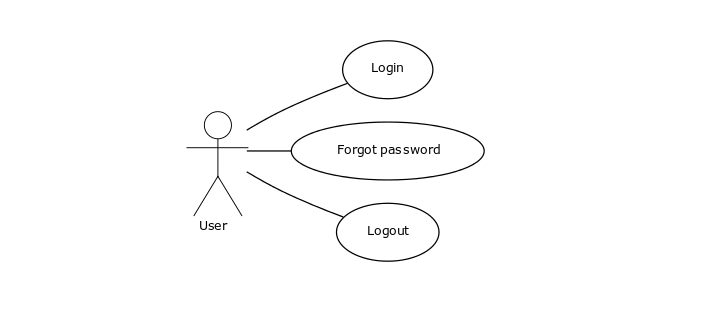
\includegraphics[scale=1]{loginout.png}


\label{UML diagram}



	

	

	\subsection{Search for and navigation to location}

\centering

\label{my-label}

\begin{tabular}{|l|l|}

\hline

\rowcolor[HTML]{EFEFEF} 

Use Case         & Searching for a location                                                                                                                                                                                                                                                                                                                                                                  \\ \hline

Description      & \begin{tabular}[c]{@{}l@{}}Type your location into the search bar in order \\ for the application to search for the \\ building/location.\end{tabular}                                                                                                                                                                                                                                    \\ \hline

Precondition     & \begin{tabular}[c]{@{}l@{}}It has to be a location inside the Hatfield \\ campus of The University of Pretoria.\end{tabular}                                                                                                                                                                                                                                                              \\ \hline

Assumption       & \begin{tabular}[c]{@{}l@{}}1. You are connected to TUKS Wi-Fi.\\ 2. You know the name of your destination\\ \\ building.\end{tabular}                                                                                                                                                                                                                                                     \\ \hline

Cases            & \begin{tabular}[c]{@{}l@{}}1. Click on the search bar and start typing\\ the \\ location you are interested in.\\ 2. If the location is not found make sure\\ \\ everything is spelled correctly.\\ 3. Choose your destination from a list of\\ \\ possible locations.\\ 4. Click on the directions link in order for the\\ \\ program to display the route to your location\end{tabular} \\ \hline

Expected results & \begin{tabular}[c]{@{}l@{}}1. After typing in the search bar the\\ location \\ you are interested in is displayed.\\ 2. You click on your destination.\\ 3. The application displays the directions from\\ \\ to point you are now to your destination.\end{tabular}                                                                                                                      \\ \hline

\end{tabular}




\centering

\label{my-label}

\begin{tabular}{|l|l|}

\hline

\rowcolor[HTML]{EFEFEF} 

Use Case         & Navigating to chosen location                                                                                                                                                                                                                                                                                                                                                         \\ \hline

Description      & \begin{tabular}[c]{@{}l@{}}The application will guide you through campus \\ towards the destination of choice, making your \\ route the shortest possible with the least \\ amount of traffic.\end{tabular}                                                                                                                                                                           \\ \hline

Precondition     & \begin{tabular}[c]{@{}l@{}}1. You are connected to TUKS Wi-Fi and have a \\ stable connection.\\ 2. You already chose your destination by \\ searching for it.\end{tabular}                                                                                                                                                                                                           \\ \hline

Assumption       & \begin{tabular}[c]{@{}l@{}}1. You are connected to TUKS Wi-Fi with a \\ stable connection.\\ 2. You know where you want to go.\end{tabular}                                                                                                                                                                                                                                           \\ \hline

Cases            & \begin{tabular}[c]{@{}l@{}}1. The application shows you the route to follow.\\ 2. You lose your Wi-Fi connection and the \\ application has to wait or  recalculate your position.\\ 3. While walking the application recalculates your \\ route based on the  traffic ahead.\\ 4. While walking the app shows your present \\ location and whether  you arrived or not.\end{tabular} \\ \hline

Expected results & \begin{tabular}[c]{@{}l@{}}1. The application shows the shortest route with \\ least amount of traffic.\\ 2. As you walk you follow along to make sure you \\ are on track.\\ 3. The application will let you know when you arrive.\end{tabular}                                                                                                                                      \\ \hline

\end{tabular}







\centering

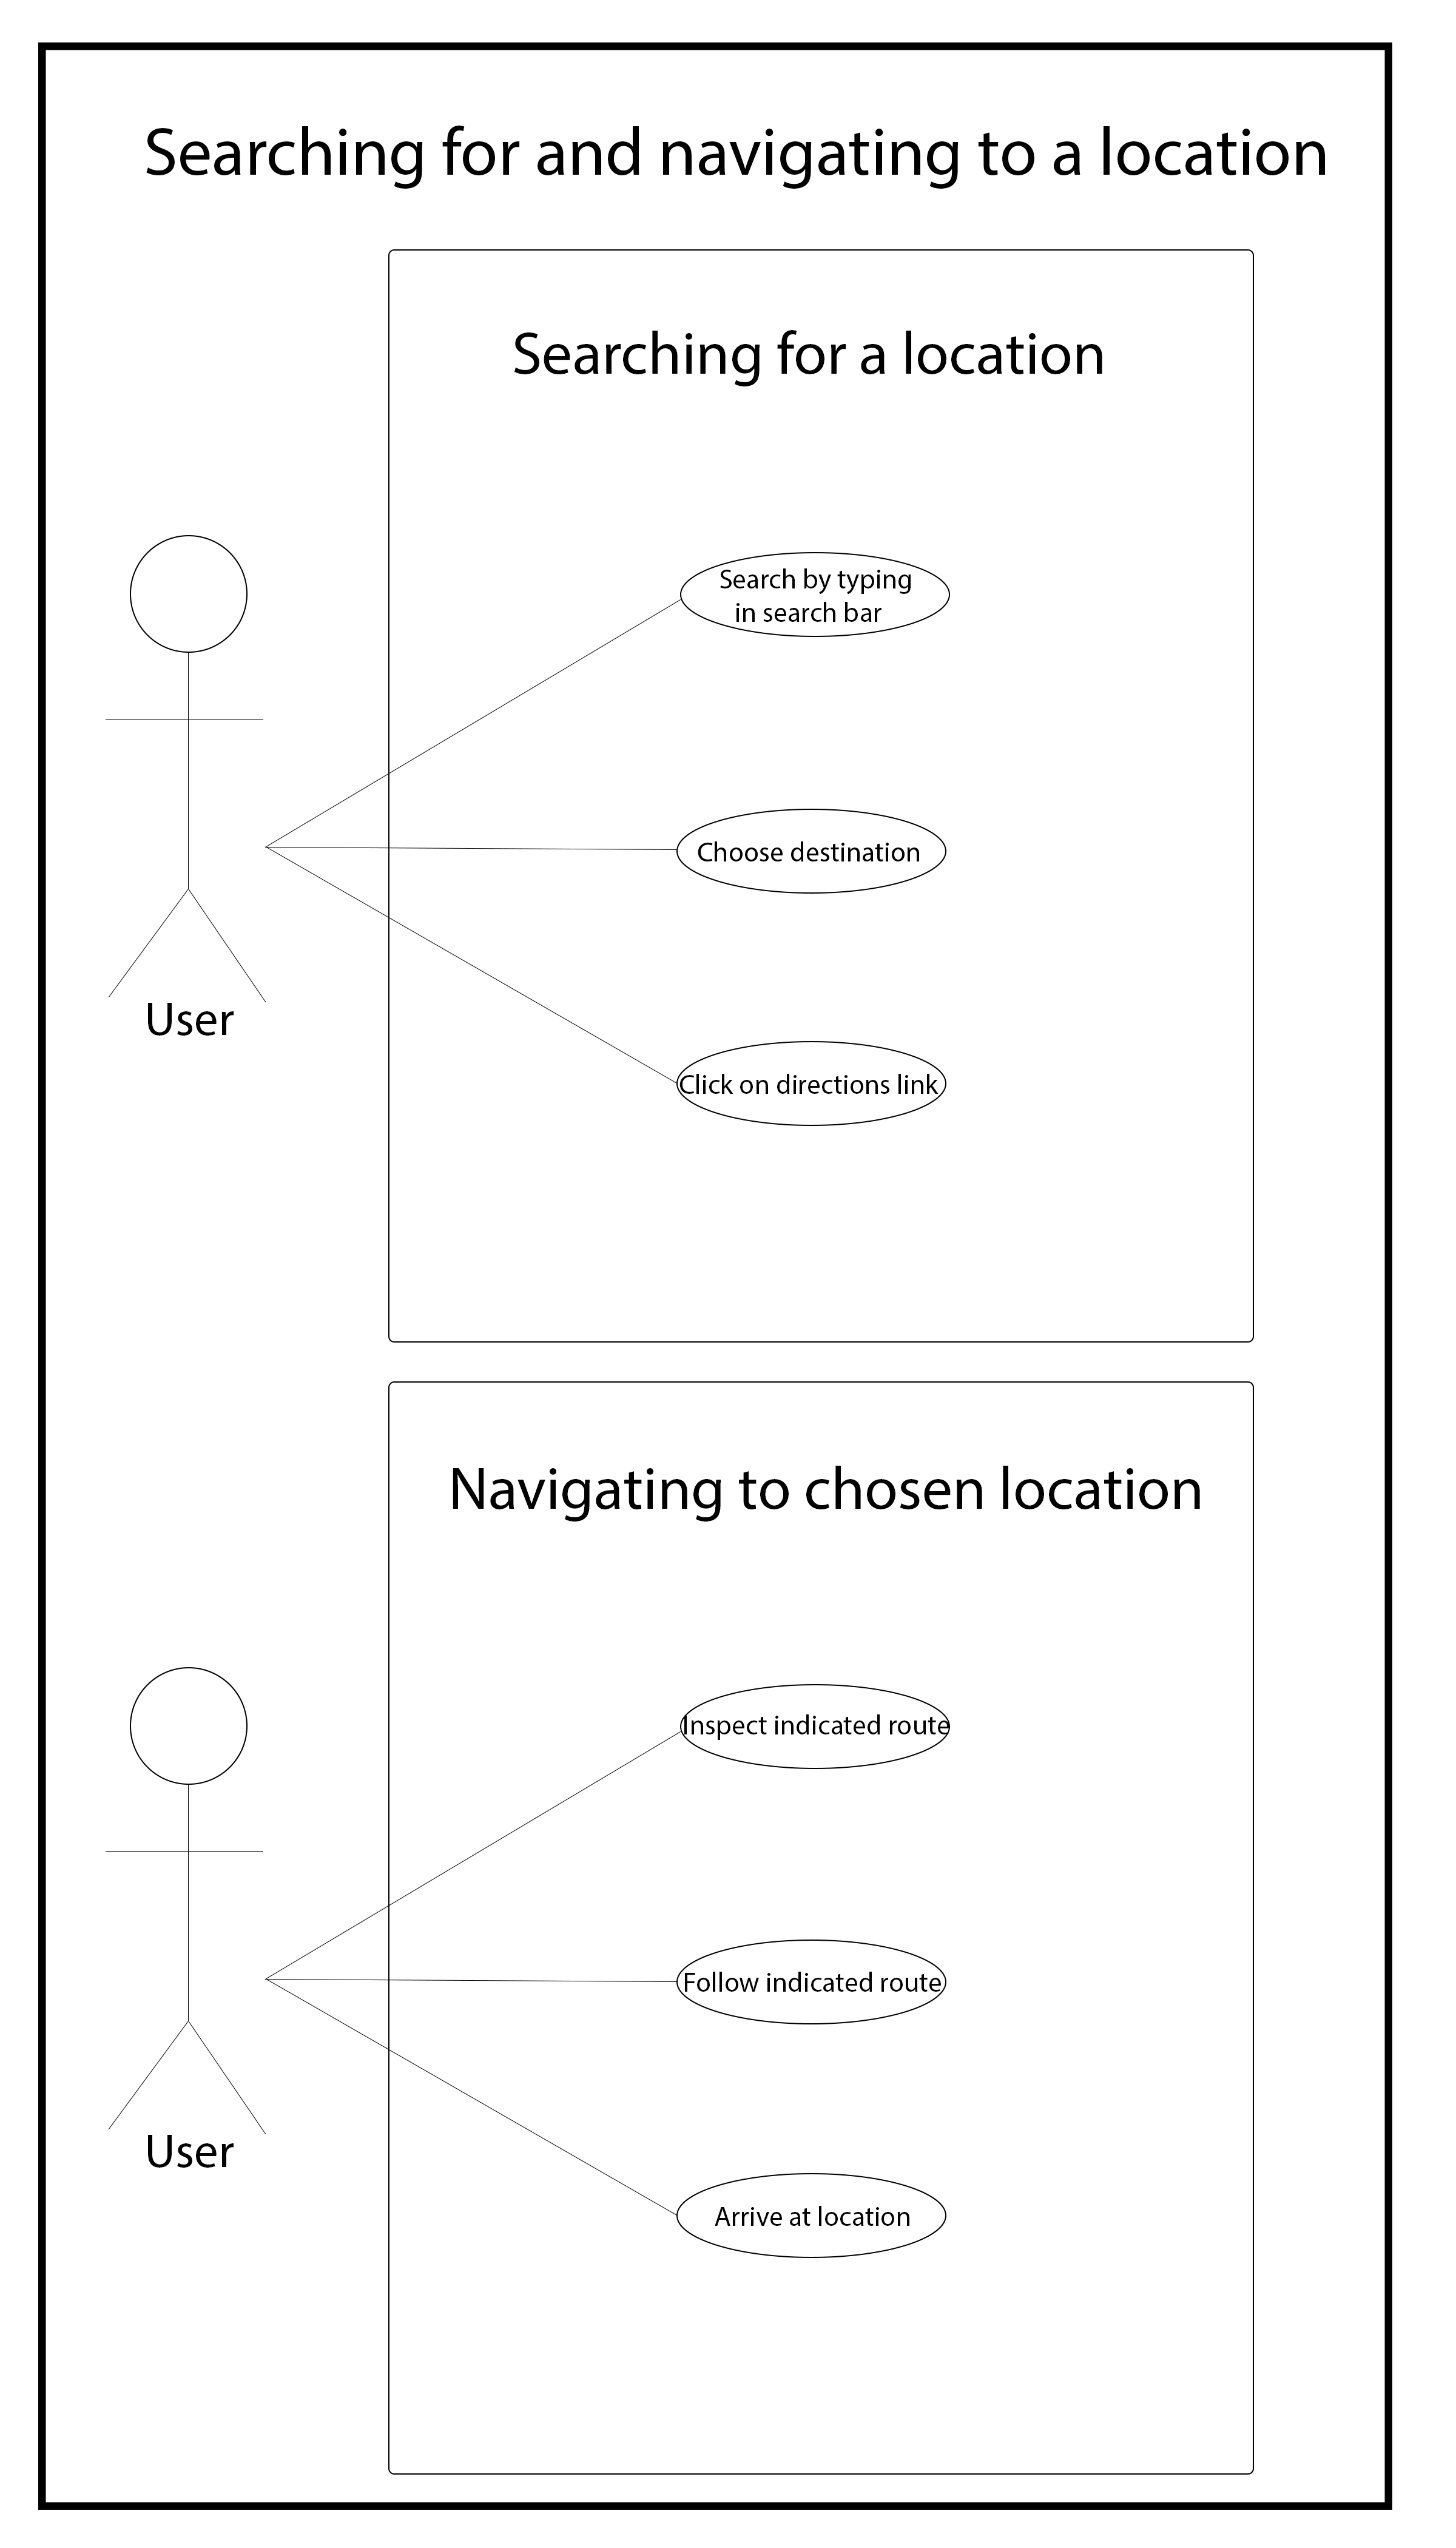
\includegraphics[scale=0.5]{SandN.png}


\label{UML diagram}



	

	

	\subsection{View Traffic Congestion}

	\begin{tabular}{|p{4cm}|p{10cm}|}

\hline



Use Case Element & Description \\

\hline



Use Case Name & 

View Traffic Congestion \\

\hline



Use Case Description & 

The user will be able to plan ahead by viewing the current traffic congestion to a desired location, and can then decide whether he or she has time to travel to that location, or would rather go at a later stage.   \\

\hline



Primary Actor & 

Student/staff/guest \\

\hline



Precondition & 

The user must be within the campus map boundaries and have an active Wi-Fi connection.   \\

\hline



Trigger & 

When the user taps on the feature to view traffic on a given route.   \\

\hline



Basic Flow & 

When the user is on the main screen of the application, the user can:

\begin{enumerate}

\item Tap on "View Traffic Congestion"

\item Pick a destination

\item Then see the approximate congestion from the user's current location to requested destination.

\end{enumerate} \\

\hline



\hline

\end{tabular}



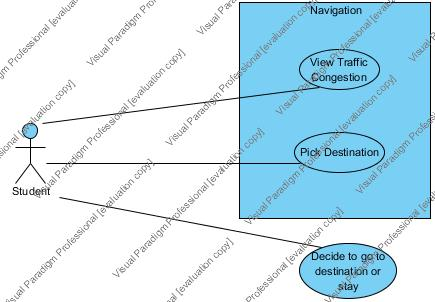
\includegraphics[width=\linewidth]{UseCaseDiagram_ViewTrafficCongestion.jpg}

View Traffic Congestion Use Case Diagram





	\subsection{Choose Route Type}

	\begin{tabular}{|p{4cm}|p{10cm}|}

\hline



Use Case Element & Description \\

\hline



Use Case Name & 

Choose Route Type \\

\hline



Use Case Description & 

The user must be able to pick from a selection of route types, be it shortest, fastest, wheelchair friendly etc.   \\

\hline



Primary Actor & 

Student/staff/guest \\

\hline



Precondition & 

The user must be within the campus map boundaries and have an active Wi-Fi connection.   \\

\hline



Trigger & 

When the user starts the process of requesting navigation instructions.   \\

\hline



Basic Flow & 

When the user is in the process of setting the conditions needed for navigation, the user will be able to:

\begin{enumerate}

\item Tap on the “Choose Route Type” drop down menu

\item Select the most appropriate option such as

	\begin{enumerate}

	\item Shortest path (Making use of actual distance from point A to B)

	\item Fastest path (Making use of heat maps to plot least congested path from point A to B)

	\item Wheelchair Friendly (Taking to account routs with Elevators and wheelchair ramps available)

	\end{enumerate}

\end{enumerate} \\

\hline



\hline



\end{tabular}



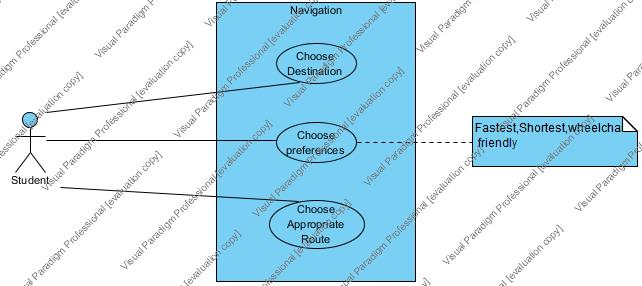
\includegraphics[width=\linewidth]{UseCaseDiagram_ChooseRouteType.jpg}

Choose Route Type Use Case Diagram



	\subsection{Home Page}

	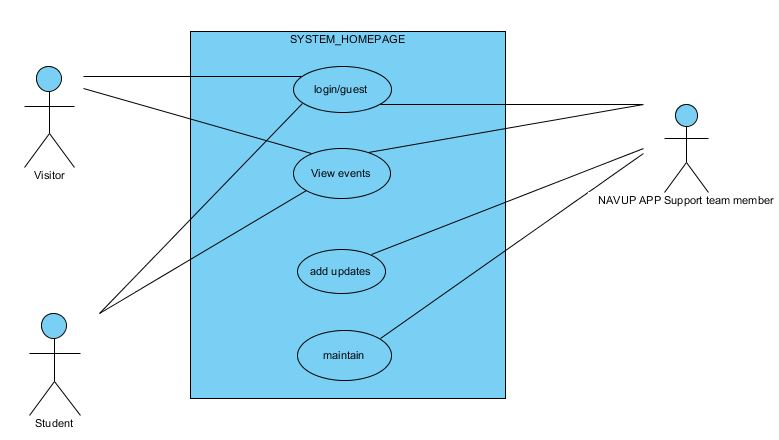
\includegraphics[width=\linewidth]{Home page.jpg}

	

	\subsection{Time Table}

	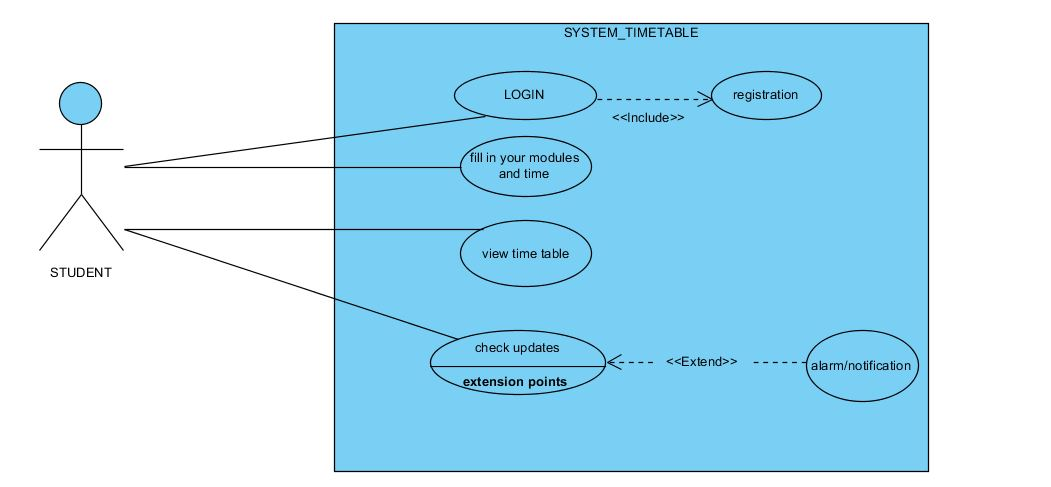
\includegraphics[width=\linewidth]{timetable.jpg}

	

	

	

	

\section{Sequence Diagrams}

	

	\subsection{Basic Functionality}

	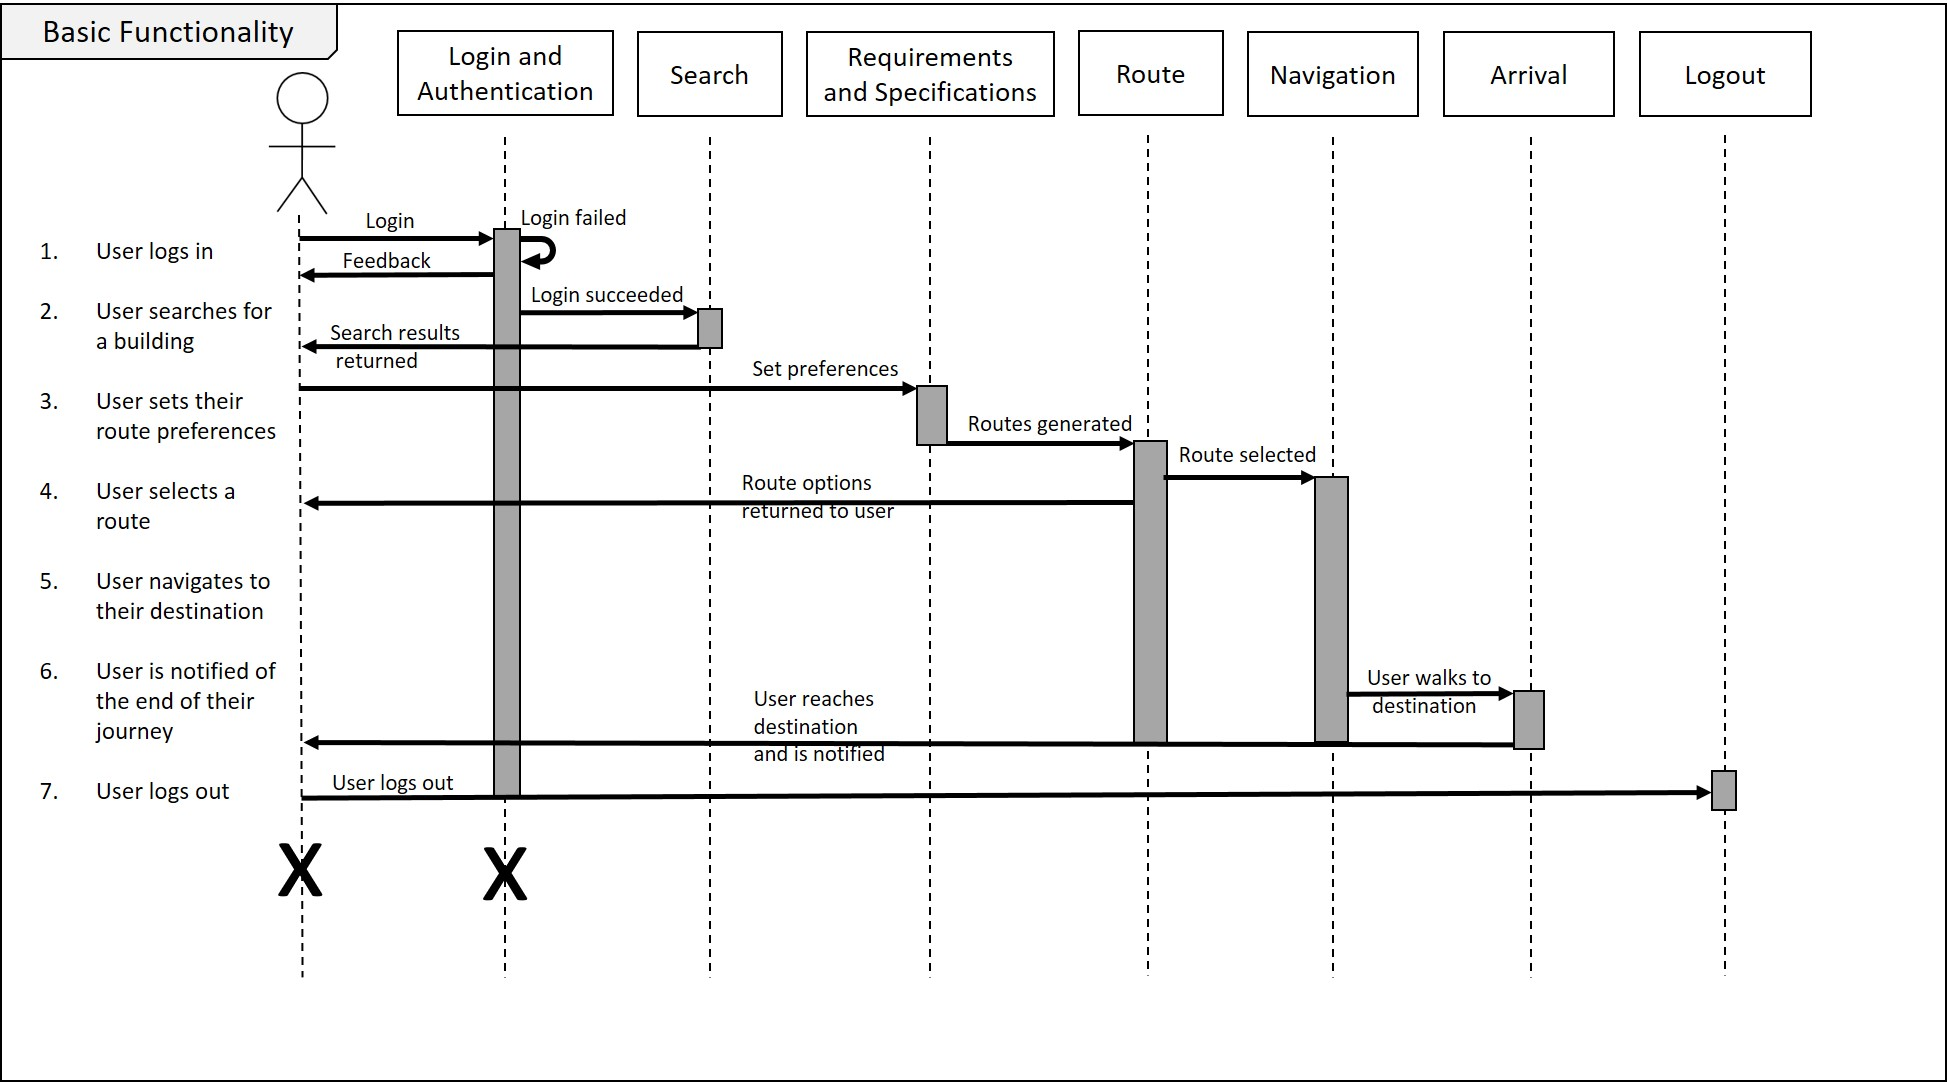
\includegraphics[width=\linewidth]{BasicFunctionality_SequenceDiagram_Schae.jpg}

	
  

\end{document}


